% \subsubsection{GeneNetWeaver}
\begin{frame}<1>[label=gnw]
\label{sec:dream}
\begin{columns}
\begin{column}{0.53\textwidth}
\alt<1>{
\frametitle{GeneNetWeaver}
\begin{itemize}
    \item Simulating gene expression in Java
    \item Used in DREAM challenge for benchmarking inference
    \item Regulation model:
\end{itemize}
% Modelling gene expression with differential equations has been applied to benchmark different attempts at inferring which transcription factors regulate which genes. The DREAM~(Dialogue for Reverse Engineering Assessments and Methods) challenges are organised by a variety of researchers from multiple organizations putting forward a challenge open to the public and assessing attempts at a solution. "DREAM4" was a challenge in reverse-engineering an in silico gene regulation network from gene expression levels. Gene expression levels were simulated, instead of collected experimentally, in order for the true underlying interactions to be definitively known.
% The simulation was intended to be biologically realistic and was simulated using the Java software GeneNetWeaver applying a nondimensionalized model defined as the differential equations in~\autoref{eq:gnw_main}, which are clearly similar to the differential equations in~\autoref{eq:Chen99}.
\begin{subequations}
\label{eq:gnw_main}
\begin{align}
\label{eq:gnw_main.a}
\dv{r_i}{t} &=  m_i^{(\text{RNA})} f_i(\boldsymbol{p}) - \lambda_i^{(\text{RNA})} r_i \\
\dv{p_i}{t} &=  m_i^{(\text{Prot})} r_i -  \lambda_i^{(\text{Prot})} p_i
\end{align}
\end{subequations}
% The values $m_i^{(\text{RNA})}$ and $m_i^{(\text{Prot})}$ are the maximum transcription and translation levels for the $i$-th protein. The function $f_i$ describes the expected fraction of maximum transcription for gene $i$ given nondimensionalized protein concentrations $\boldsymbol{p}$, so it holds $f_i(\boldsymbol{p}) \in [0,1]$.
% $f_i$ is mentioned in supplementary material of~\cite{Marbach2010} and based on the work in~\cite{GeneNetWeaverModel}. It takes into account different types of gene regulation, both regulator interactions and cooperation for any combination of activators and repressors~(\autoref{fig:gnw_regulation}).
% A gene has a set of binding sites, each affecting its transcription level. Each of the TFs regulating gene $i$ can bind to only one binding site in the GeneNetWeaver model. The TF can bind to the binding site with dynamics built on Hill equations~(\autoref{eq:Hill}). The effect of a bound site on gene transcription rate can be flipped in the model, indicated for site $m=2$ in~\autoref{fig:gnw_regulation}, where TFs binding the site using dynamics inspired by activator Hill equations~(\autoref{eq:Hill_activator}) has a repressing effect on the transcription rate of gene $i$.
}{
\stepcounter{equation}
}
\only<2>{
\frametitle{GeneNetWeaver - Example}
% The terms defined in~\autoref{eq:gnw_f} are calculated using the example shown in~\autoref{fig:gnw_regulation} for illustrative purposes:
\begin{subequations}
\begin{align*}
N &= 3
\,,\,
C = \{3\}
\\
A_1 &= \{1\}
\,,\,
A_2 = \{4\}
\,,\,
A_3 = \{5,6\}
\\
R_1 &= \emptyset
\,,\,
R_2 = \{2,3\}
\,,\,
R_3 = \emptyset
\\
\mu_1 &= \frac{\chi_1}{1 + \chi_1}
\\
\mu_2 &= \frac{\chi_4}{1 + \chi_4 + \chi_2 \chi_3 \chi_4}
\\
\mu_3 &= \frac{\chi_5}{1 + \chi_5} \frac{\chi_6}{1 + \chi_6}
\\
\sigma_1 &= \emptyset
\,,\,
\sigma_2 = \{1\}
\,,\,
\sigma_3 = \{2\}
\,,\,
\sigma_4 = \{1,2\}
\\
\sigma_5 &= \{3\}
\,,\,
\sigma_6 = \{1,3\}
\,,\,
\sigma_7 = \{2,3\}
\,,\,
\sigma_8 = \{1,2,3\}
\\
P\{\sigma_1 | \boldsymbol{p}\} &= (1 - \mu_1) (1 - \mu_2) (1 - \mu_3)
\\
P\{\sigma_2 | \boldsymbol{p}\} &= \mu_1 (1 - \mu_2) (1 - \mu_3)
\\
P\{\sigma_3 | \boldsymbol{p}\} &= (1 - \mu_1) \mu_2 (1 - \mu_3)
\\
...
\\
P\{\sigma_8 | \boldsymbol{p}\} &= \mu_1 \mu_2 \mu_3
\end{align*}
\end{subequations}

}
\end{column}
\begin{column}{0.47\textwidth}

\begin{figure}[ht]
  \centering
  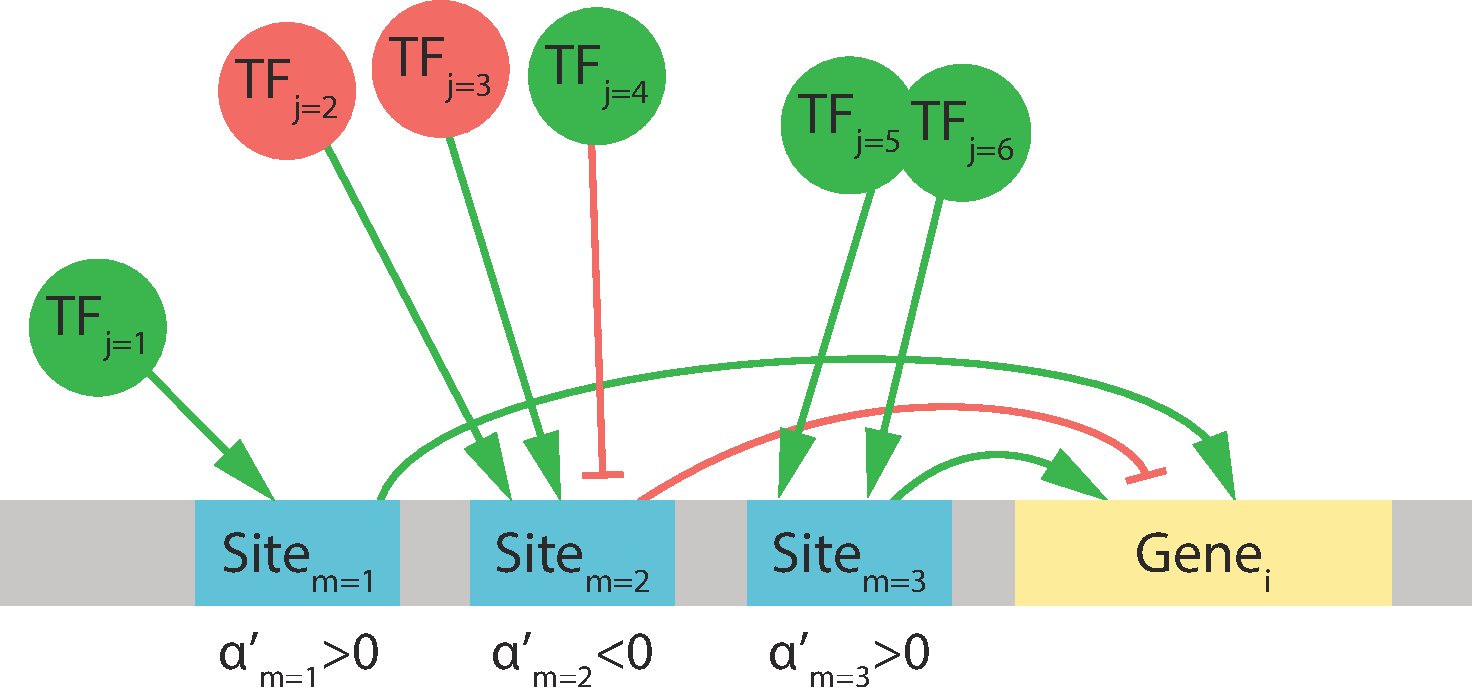
\includegraphics[width=\textwidth]{theory/fig/GeneWeaverRegulation.pdf}
   \caption{\textbf{Example of transcriptional regulation in simulation.}
    A gene regulated by $N=3$ regulatory modules, where module 1 is regulated by a single activator TF, module 2 is bound by a complex of two TFs, which both have to be present for activation of the module, and activating and repressing TFs compete to bind the third module. \textcolor{OliveGreen}{Green}: activation, \textcolor{red}{red}: repression.} 
  \label{fig:gnw_regulation}
\end{figure}



\end{column}
\end{columns}
\end{frame}

\begin{frame}{GeneNetWeaver - Defining gene regulation}
\begin{columns}
\begin{column}{0.5\textwidth}
% The exact equation for $f$ is unpublished but defined in the source code, and written here in~\autoref{eq:gnw_f}, focusing on the function $f_i$ for a single gene $i$. Each binding site can either be bound by transcription factor(s) or unbound. For $N$ binding sites this creates $2^N$ unique combinations~(\autoref{eq:gnw_f.a}), which we refer to as "states". Each state~$\sigma_s$ for $s \in \{1,2,3,...,2^N\}$ are each defined as a unique combination of bound and unbound binding sites.
\small
Based on Marbach~et~al.~\cite{Marbach2010}, Dassow~et~al.~\cite{GeneNetWeaverModel}
\normalsize
\begin{subequations}
\label{eq:gnw_f}
\begin{align}
\label{eq:gnw_f.a}
f_i(\boldsymbol{p}) &=
\sum_{s=1}^{2^N} \alpha_s P\{\sigma_s | \boldsymbol{p} \}
\\
\label{eq:gnw_f.b}
\alpha_s &=
\alpha_0' + \sum_{m \in \sigma_s} \alpha_m'
\\
\label{eq:gnw_f.c}
P\{\sigma_s | \boldsymbol{p} \} &=
\prod_{m \in \sigma_s} P\{\beta_m=1|\boldsymbol{p}\} \cdot \prod_{m \notin \sigma_s} \left( P\{\beta_m=0|\boldsymbol{p}\} \right)
\\
\label{eq:gnw_f.d}
&=
\prod_{m \in \sigma_s} \mu_m \cdot \prod_{m \notin \sigma_s} \left( 1 - \mu_m \right)
\end{align}
\end{subequations}
$\beta_m$ = module $m$ under activating binding conditions
\end{column}

\begin{column}{0.5\textwidth}
\begin{subequations}
\begin{align}
\label{eq:gnw_f.e}
\mu_m &=
\begin{cases}
  \frac{\prod_{j \in A_m} \chi_j}{\prod_{j \in A_m \vee R_m} 1 + \chi_j},
  & \text{if}\ m \in C \\
  \frac{\prod_{j \in A_m} \chi_j}{1 + \prod_{j \in A_m} \chi_j},
  & \text{if}\ m \notin C \wedge \forall j \in A_m \\
  \frac{\prod_{j \in A_m} \chi_j}{1 + \prod_{j \in A_m} \chi_j + \prod_{j \in A_m \vee R_m} \chi_j},
  & \text{otherwise}
\end{cases}
\\
\label{eq:gnw_f.f}
\chi_j &=
\left( \frac{p_j}{k_j} \right) ^ {\nu_j}
\end{align}
\end{subequations}
% Here, $P\{\sigma_s | \boldsymbol{p}\}$ is the probability that a gene is in regulation state $\sigma_s$ given the current protein concentrations $\boldsymbol{p}$. $\alpha_s$ is the fraction of maximum gene transcription for state~$\sigma_s$, and is computed from the sum of baseline activation and relative activation for each binding site that are bound in the given state $\sigma_s$~(\autoref{eq:gnw_f.b}). It holds $\alpha_s \in [0,1]$.
% If we consider state $\sigma_s$ a set of all binding sites bound when a gene is in said state, then the probability that gene $i$ is in state $\sigma_s$ is defined by the probability of sites in set $\sigma_s$ bound and sites not in $\sigma_s$ unbound~(\autoref{eq:gnw_f.c}). The Boolean $\beta_m$ indicates if site $m$ is bound or not. The probabilities are equivalent to the expected fraction of binding sites bound~(\autoref{eq:gnw_f.d}), which is defined in three different ways in~\autoref{eq:gnw_f.d} depending on whether the binding site is regulated by a TF binding complex~($m \in C$), and if some of the TFs for a binding site are repressors~($\exists j \in R_m$) or if all are activators~($\forall j \in A_m$).
% \autoref{eq:gnw_f.e} is based on Hill equations~(\autoref{eq:Hill}). It can be seen that if a binding site $m$ is only regulated by a single activating TF, then we get $\mu_m = \theta_{\text{activator}}$ from \autoref{eq:Hill_activator} and if only regulated by a single repressing TF, we get $\mu_m = \theta_{\text{repressor}}$ for \autoref{eq:Hill_repressor}. This is the case regardless if $m \in C$ or not, although it does not make sense to describe a lone transcription factor as regulating in a complex.
% \pagebreak
\end{column}
\end{columns}
\end{frame}

\againframe<2>{gnw}

\begin{frame}{GeneNetWeaver - Initial conditions}
% To prepare for the simulation, the GeneNetWeaver software is given an adjacency matrix~(\autoref{sec:graph}) with values indicating which genes each protein regulates. Model parameters are then set randomly, for instance setting random mRNA and protein decay rates. Rate parameters are assigned random values using~\autoref{eq:gnw_param_initial} which describes random decay rates.

\begin{subequations}
\label{eq:gnw_param_initial}
\begin{align}
m_i^{(\text{RNA})} &= \lambda_i^{(\text{RNA})} \sim \frac{\log (2)}{\mathcal{T}(a=5, b=50)} \\
m_i^{(\text{Prot})} &= \lambda_i^{(\text{Prot})} \sim \frac{\log (2)}{\mathcal{T}(a=5, b=50)}
\end{align}
\end{subequations}

$\mathcal{T}(a,b)$ = normal distribution truncated to $[a,b]$. $a$ and $b$ selected from~\cite{GeneNetWeaverModel}


$\mathcal{T}(a,b)$ has $\mu=\frac{a+b}{2}$, $\sigma=\frac{b-a}{6}$



% Here, $\mathcal{T}(a,b)$ is a normal distribution truncated to the interval $[a,b]$ with $\mu=\frac{a+b}{2}$ and $\sigma=\frac{b-a}{6}$. It serves as descriptor of mRNA and protein half-life. Its range parameters are selected based on~\cite{GeneNetWeaverModel}.


% Gene expression and protein levels are initialized at time zero by letting gradients equal zero as described in~\autoref{eq:initial_gnw}.

\begin{subequations}
\label{eq:initial_gnw}
\begin{align}
\dv{r_i}{t} = 0 &\implies r_i = \frac{m_i^{(\text{RNA})}}{\lambda_i^{(\text{RNA})}}  f_i(\boldsymbol{p})  \\
\dv{p_i}{t} = 0 &\implies p_i = \frac{m_i^{(\text{Prot})}}{\lambda_i^{(\text{Prot})}} r_i
\end{align}
\end{subequations}

% Gene expressions $r_i$ for each gene $i$ are initially set without protein regulation, which means $r_i$ is evaluated here using $\boldsymbol{p} = \boldsymbol{0}$. More initialization code is also run in order to set $\alpha_s$ for each state.


\end{frame}